 \setlength{\footskip}{1cm} 

\subsection*{\Large Общая характеристика работы}
\fontsize{14pt}{15pt}\selectfont

\textbf{Актуальность проблемы.}  Разработка эффективных вычислительных  методов решения информационных задач является важнейшим направлением развития современных информационных технологий (и в целом, прогресса, так как невозможно представить современную науку,  технику  и общественную жизнь без использования компьютеров). 
В идеале, эти методы должны обеспечивать скорость решения ряда важных информационных задач вне зависимости от объема данных. И действительно, есть ряд важных  информационных задач, где это возможно. 

Наглядным (и очень важным) примером  этого являются реляционные базы данных (БД), где вычислимость запросов определенных типов не зависит от объема данных, а только линейно от сложности проекта самой БД.

Практическим подтверждением этого для обывателя является скорость работы банковских систем, использующих сетевые реляционные БД,  с их мировыми сетями терминалов и банкоматов, где можно проводить операции с вкладами и денежными средствами в любой точке мира за считанные секунды.

Отметим, что весьма близко к этому классу  примыкают задачи поиска данных по ключевым словам в Интернет - пространстве (полно текстовые поисковые системы «Google», «Яндекс» и др.), где скорость поиска не замедляется из-за экспоненциального роста информации в глобальной сети.

Другим  важным классом информационных задач являются вопросы распознавания  образцов (образов), где при организации данных близкой к таблицам реляционных БД также могут быть получены результаты независимости скорости  распознавания  образцов от их количества, вернее, верхней границы сложности распознавания одного образца с добавкой только количества образцов. 

Данное направление исследований (разработка эффективных вычислительных  методов решения информационных задач) весьма актуально для современной  науки в целом и техники, как в теоретическом, так и  практическом плане, где работают крупные транснациональные компьютерные корпорации, реализуются технологии «Big Table»,  «Big Data» и предполагается получение прорывных результатов в робототехнике, молекулярной биологии, системах искусственного интеллекта и других важных областях, имеющих определяющее значение для прогресса современного общества.

В диссертационной работе рассматриваются вопросы анализа контурных изображений (поиск образцов в изображении), получены оценки алгоритмической сложности такого анализа (близкие к аналогичным результатам для табличной организации данных), созданы программные комплексы решающие прикладные задачи.
Предложенные в  диссертационной работы методы и полученные результаты являются продолжением исследований: 
- Д.Кнута и др. по эффективной вычислимости запросов для данных, представленных древовидными структурами;
- Э.Кодда и др. по табличной организации данных для реляционных сетевых СУБД (MS SQL Server, Oracle и др., включая технологии «Big Table»).
%(Миша вставьте тут про обработку растровых данных или еще что. Да и надо сноски делать с пропиской лит-ры. Да, еще из интернета подставьте параметры Совета по БГУ искать)

В принципиальном плане результаты диссертационной работы могут интерпретироваться как возможность получения для технологий «Big Data» по анализу изображений практически таких же эффективных методов, как  технологии  «Big Table» для табличной организации данных.

\textbf{Целью данной работы} является построение  моделей контурных изображений, которые, хотя и имеют более сложную организацию данных, чем  таблицы реляционных БД, но позволяют получить почти аналогичные результаты по вычислительной сложности  анализа контурных изображений, включая проверку изоморфных вложений образцов в анализируемое изображение.

Разработка новых  методов моделирования объектов и явлений  в диссертации представлена результатами по построению  моделей контурных изображений.
Разработка, обоснование и тестирование эффективных вычислительных методов с применением современных компьютерных технологий в диссертации представлена результатами по эффективной вычислимости анализа, полученных  моделей контурных изображений, включая проверку изоморфной вложимости совокупности контурных изображений (образцы) в исследуемое контурное изображение.

Реализация эффективных численных методов и алгоритмов в виде комплексов проблемно-ориентированных программ для проведения вычислительного эксперимента в диссертации представлена результатами по применению комплексов программ для решения конкретных прикладных задач  (см. Приложения).


\textbf{Для достижения поставленной цели необходимо было решить следующие задачи:}

\begin{enumerate}
\item Разработать алгоритмы преобразование растра контурного изображения в нагруженный граф специального вида.
\item Разработать преобразование нагруженных графов специального вида в математические модели, представленные многоосновными алгебраическими системами, где контурные изображения сведены к ориентированным дугам, связям дуг и их численным характеристикам в градусном измерении и  относительных размеров  длины дуг.
\item Исследовать алгоритмическую сложность  анализа контурных изображений, включая проверку изоморфных вложений образцов в анализируемое изображение, где контурные изображения сведены к ориентированным дугам, связям дуг и их численным характеристикам в градусном измерении и  относительных размеров  длины дуг.
\item Разработать  масштабные ряды контурных изображений и процедуры сжатия на  основе относительных размеров дуг.
\item Исследовать возможность использования  изоморфного вложения сжатого образца в сжатое изображение для уменьшения алгоритмической сложности построения  изоморфного вложения исходного образца в исходное изображение.
\item Исследовать возможность использования полученных математических методов, математических моделей представления данных, алгоритмов и комплексов программ для решения прикладных задач:
 \begin{enumerate}
 \item распознавания символов; 
 \item оценки устойчивости битумных эмульсий;
 \item автоматизации составления проектов организации дорожного движения (ПОДД).
 \end{enumerate}
\end{enumerate}
 
\textbf{Основные положения, выносимые на защиту:}

\begin{enumerate}
\item Сходящийся алгоритм волновой скелетизации,  обеспечивающий преобразование растра контурного изображения в нагруженный граф специального вида (Утверждение 2.3.1.).
\item Оценка нижней границы алгоритмической сложности  анализа контурных изображений, включая проверку изоморфных вложений образцов в анализируемое изображение, где контурные изображения сведены к ориентированным дугам, связям дуг и их численным характеристикам в градусном измерении и  относительным размерам  длины дуг  (Теорема 2.5.1.).
\item Масштабные ряды плоских контурных изображений и их применение для уменьшения  вычислительной сложности анализа контурных изображений.  (Теоремы 1, 2, 3.).
\item Комплексы программ  решения прикладных задач:
 \begin{enumerate}
   \item распознавания символов;
   \item оценки устойчивости битумных эмульсий;
   \item автоматизации составления проектов организации дорожного движения (ПОДД). 
 \end{enumerate}
\end{enumerate}   

\textbf{Научная новизна:}

\begin{enumerate}
\item Впервые построены математические модели контурных изображений, представленных ориентированными дугами, связям дуг и их численными характеристиками в градусном измерении,  а также  относительными размерами  длин дуг.  
\item Впервые  показано, что математические модели контурных изображений, хотя и имеют более сложную организацию данных, чем  таблицы реляционных БД, но позволяют получить почти аналогичные результаты по алгоритмической сложности  анализа контурных изображений, включая проверку изоморфных вложений образцов в анализируемое изображение.
\item Было выполнено оригинальное исследование использования масштабных рядов контурных изображений и процедуры сжатия на  основе относительных размеров дуг, которые можно использовать для повышения эффективности анализа исходных изображений.
\end{enumerate}   

\noindent
\textbf{Научная и практическая значимость определяется:}

\begin{enumerate}
\item Во-первых, актуальностью направления исследований, которое обеспечивает применение информационных технологий буквально во всех сферах современной деятельности общества;

\item Во-вторых, применением разработанных программных комплексов для решения прикладных задач, что подтверждено официальными справками о применении результатов диссертации.
\end{enumerate}

\textbf{Степень достоверности полученных результатов обеспечивается} строгими математическими формулировками определений, а также строгими математическими доказательствами полученных утверждений, лемм и теорем.

\textbf{Результаты находятся в соответствии с результатами}, полученными другими авторами: А.И.Мальцевым,  Ю.Л.Ершовым, С.В.Яблонским,  А.И.Кокориным, А.В.Манциводой,  Е.Коддом, Д.Кнутом, В.И.Мартьяновым, Д.В.Пахомовым, В.В.Архиповым и др.

\pagebreak
\textbf{Апробация работы.} Основные результаты работы докладывались на: 

\begin{enumerate}
\item ежегодных научно-теоретических конференциях аспирантов и студентов:  Иркутский  гос. университет, ИМЭИ, 2010-13 гг.
\item 3-ей Российской школе – семинаре «Синтаксис и семантика логических систем». Иркутск, 2010.
\item 4-ой Международной конференции «Математика, ее приложения и математическое образование (МПМО’11),  Улан-Удэ, 2011.
\item семинарах кафедр ИГУ, ИРНИТУ, ИрГУПС, 2010-17гг.
\item межрегиональных конференциях "Платоновские чтения – 2015-17гг."
\end{enumerate}


\textbf{Личный вклад.} Автором получены самостоятельно результаты основных положений 1, 2, 6,  выносимых  на защиту.  Результаты основных положений 3, 4, 5,  выносимых  на защиту, получены в нераздельном соавторстве с В.И. Мартьяновым, которому принадлежит начальное определение масштабных рядов контурных изображений и предложение их использования для уменьшения вычислительной сложности анализа контурных изображений.

\textbf{Публикации.} Результаты диссертационного исследования
опубликованы в 12 научных работах, в том числе 9 работ в рецензируемых научных изданиях, рекомендованных ВАК РФ. Получены свидетельства о государственной регистрации программ для ЭВМ.
Все вносимые на защиту результаты получены лично автором или при его непосредствен-
ном участии.

\textbf{Структура и объем работы.} Диссертация состоит из введения, трех глав, заключения и двух приложений. Полный объем диссертации составляет 106 страница с 29 рисунками и 7 таблицами. Список литературы содержит 40 наименований.

\subsection*{\Large Содержание работы}
Во введении показана актуальность и практическая значимость представленных в настоящей работе исследований, приведена информация о внедрении и апробации работы.

\textbf{Первая глава} содержит описание современного состояния теории распознавания образов, работы поисковых систем, а так же описание основных используемых методов и технологий. Глава состоит из 4 разделов. 

Первый раздел называется <<Теория распознавания образа>> и содержит основные понятия теории,  классическую постановка задачи, и базовую модель.

Второй раздел называется <<Распознавание текста>> и конкретизирует обобщенную постановку задачи указанную в предыдущем параграфе. В тексте делается упор на описание наиболее популярных систем распознавания печатного текста, их эффективность а также упоминаются две основных постановки задачи как задача офлайн распознавания текст (как распознавание текста на статическом изображении) и задача онлайн распознавания текста (так называемое распознавание <<на лету>>, когда система имеет возможность отслеживать процесс написания символов).

В третьем разделе рассматривается задача распознавания рукописного текста. Рассмотрены основные системы распознавания рукописного текста, их возможности и эффективность. Приведенны основные подходы используемые для решения поставленной задачи, которые включают в себя 

\begin{enumerate}
\item  <<Шаблонные методы>> -- которые преобразуют изображение отдельного символа в растровое представление, сравнивают его со всеми шаблонами, имеющимися в базе и выбирают шаблон с наименьшим количеством точек, отличных от входного изображения.

\item <<Структурные методы>> -- Структурные методы [6, 27] представляют объект как граф, узлами которого являются элементы входного объекта, а дугами – пространственные отношения между ними. Методы, реализующие подобный подход, обычно работают с векторными изображениями.

\item <<Признаковые методы>> -- Признаковые методы базируются на том, что изображению ставится в соответствие N-мерный вектор признаков. Распознавание заключается в сравнении его с набором эталонных векторов той же размерности.
\end{enumerate}

\noindent
Делается заключение о неполноте и ограниченности применения каждого метода по отдельности. В современных системах распознавания обычно используются все три типа классификаторов, но основным является структурный. Два других служат для ускорения и повышения качества распознавания. Комбинация различных методов распознавания приводит к наилучшим результатам. Параграф содержит таблицу сравнения методов.

Последний раздел содержит описание технологии BigTable.

\textbf{Вторая глава} посвящена методам решению  задачи распознаванию контурных изображений в различных вариациях и содержит описание математической модели.

Глава в целом построена в соответствии со схемой используемой при распознавании изображения.
 
Первый раздел содержит базовые определения необходимые при анализе растрового изображения.
 
Второй раздел содержит описание модели растрового изображения, которое представляет собой алгебраическую систему следующего вида:

\begin{equation}
\mathfrak{M} = < A, R, V, M; Sector, Angle, Metric, Relation >
\label{eq:model}
\end{equation}

\noindent
где
\begin{enumerate}
\item[] $A$ -- множество всевозможных дуг,
\item[] $R$ -- множество связей дуг,
\item[] $V \subset Z$ -- множество допустимых углов (например от 0 до 360 градусов),
\item[] $M \subset Z$ -- множество относительных мер,
\item[] $Sector: A \rightarrow V$ -- задает градусную меру дуги,
\item[] $Metric: A \rightarrow M$ -- функция сопоставляющая каждой дуге ее относительную величину,
\item[] $Angle: R \rightarrow V$ -- задает угол соединения двух дуг
\item[] $Relation: R \rightarrow A \times A$ -- сопоставляет каждой связи дуги, те дуги, которые она соединяет.
\end{enumerate}

Третий раздел посвящен описанию <<Волнового>> алгоритма позволяющего осуществить преобразование растрового бинарного изображения в соответствие с моделью \ref{eq:model}. Идея алгоритма заключается в генерации волны в одной из заполненных точек растрового изображения, которая проходит по изображения и позволяет построить граф (скелет) который визуально соответствует заполненной области (Рис. \ref{fig:special}). Далее этот граф разбивается на простые пути по узлам особого вида. И на конечном этапе простые пути аппроксимируются дугами, а между дуг уже расчитываются углы соединения дуг (Рис. \ref{fig:geometry})

\begin{figure}[h]

\centering
	\begin{subfigure}[centerlast,FIGBOTCAP]{.45\textwidth}
		\centering
		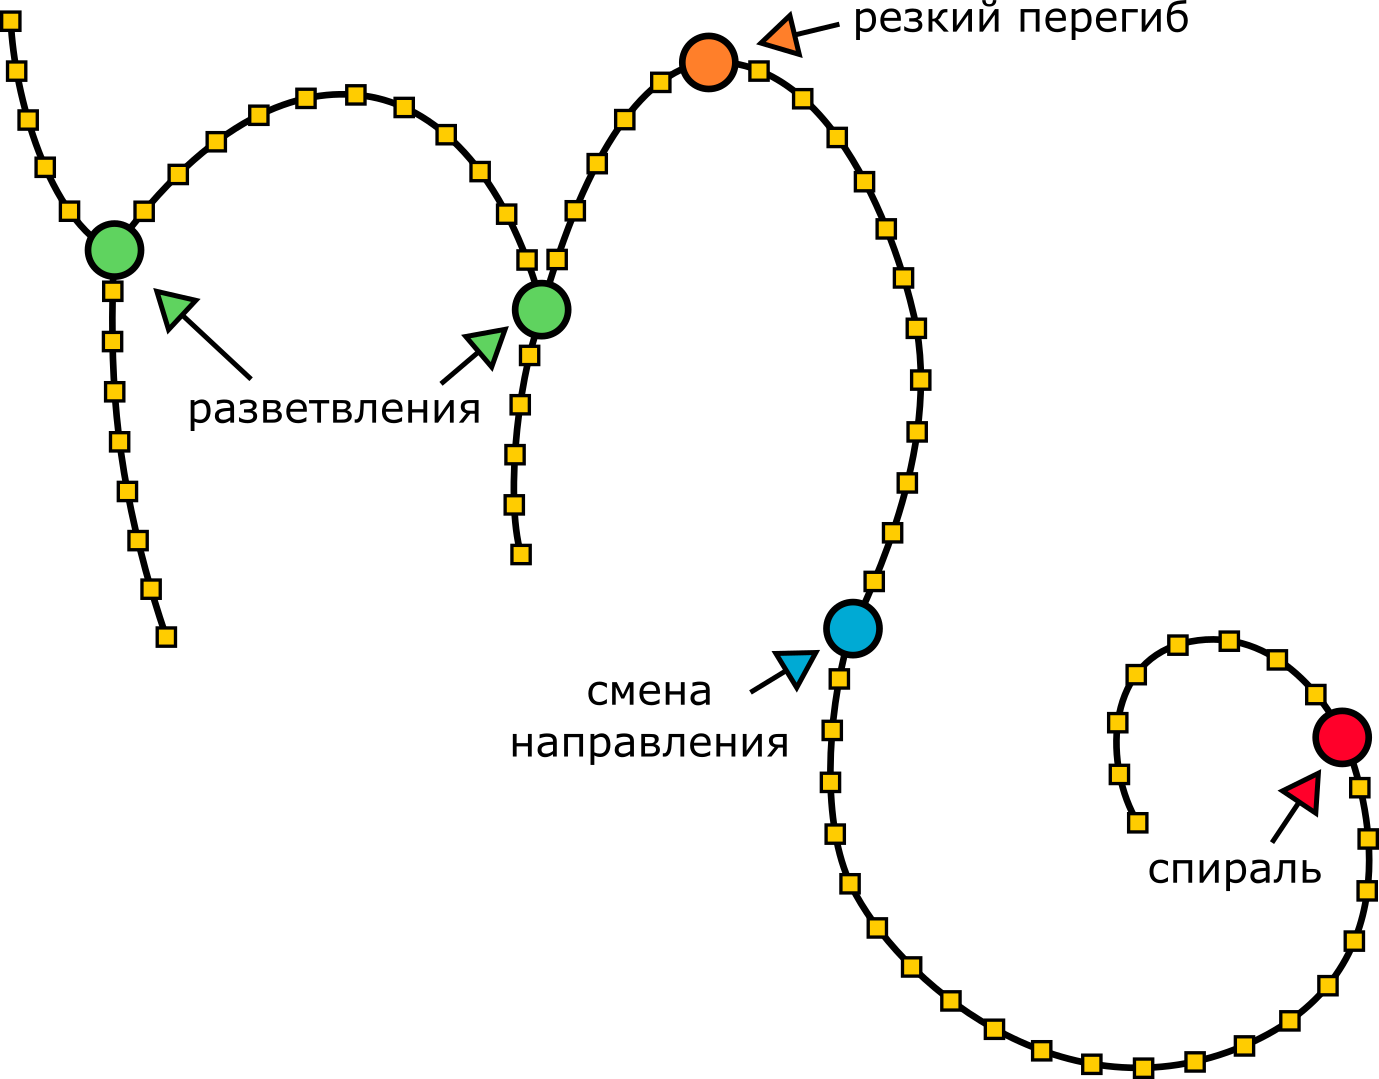
\includegraphics[width=\textwidth,keepaspectratio]{images/graph}
		\medskip
		\caption{Схема разбиения графа «особыми» точками}
		\label{fig:special}
	\end{subfigure}
	\hfill
	\begin{subfigure}[centerlast,FIGBOTCAP]{.45\textwidth}
		\centering
		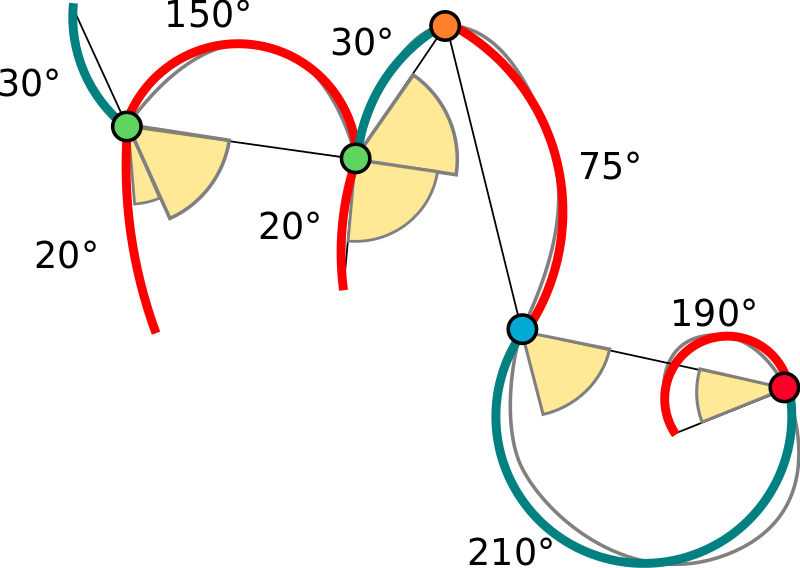
\includegraphics[width=\textwidth,keepaspectratio]{images/items}
		\medskip
		\caption{Геометрическая интерпретация модели $\mathfrak{M}$}
		\label{fig:geometry}
	\end{subfigure}
	\caption{Представление изображения}
\end{figure}

Следующий раздел содержит базовую постановку задачи распознавания, которая может быть представлена следующим образом. Пусть изображение есть модель следующего вида:
\begin{equation}
\mathfrak{M} = < A, R, V; Sector, Angle, Relation >
\label{vipeq1}
\end{equation}
\begin{equation}
M_{ini} = <A_1,...,A_s;f_1,...,f_n;p_1,...,p_k>
\label{vipeq2}
\end{equation}

Пусть многоосновные а.с.
\begin{equation}
	\begin{array}{c}
	R_1=<Arc_1, Rel_1, V; Sector, Angle, R> \\
	R_2=<Arc_2, Rel_2, V; Sector, Angle, R> \\
	\dots\\
	R_m=<Arc_m, Rel_m, V; Sector, Angle, R> \\
	\end{array}
	\label{vipeq3}
\end{equation}
задают искомые образцы в анализируемом изображении~\ref{vipeq1}.

Анализ изображения~\ref{vipeq1} состоит в поиске всех изоморфных вложений ${ \mu_{i,j} }$ многоосновных а.с. $R_1,R_2,...,R_m$ в многоосновную а.с. $\mathfrak{M}$~\ref{vipeq1}, т.е. изоморфное вложение $\mu_{i,j} : R_i \rightarrow \mathfrak{M}$ состоит из инъективных отображений
\begin{equation}
\mu_{i,j} : Arc_i \rightarrow Arc; \mu_{i,j} : Rel_i \rightarrow Rel
\label{vipeq4}
\end{equation}

\noindent
такие, что:

\begin{enumerate}
\item[а)] если $\mu_{i,j}(Ar) = Arr$,где $Ar \in Arc_i$, $Arr \in Arc$, $Sector(Ar) = (v_1, v_2)$, $Sector(Arr) = (v_3, v_4)$, то $v_1 \le v_3 \le v_4 \le v_2$;
\item[б)] если $\mu_{i,j}(Re) = Ree$, где $Re \in Rel_i$, $Ree \in Rel$, $Angle(Re) = (v_1, v_2)$, $Angle(Ree) = (v_3, v_4)$, то $v_1 \le v_3 \le v_4 \le v_2$;
\item[в)] если $R(Re, Ar_1, Ar_2)$, где $Re \in Rel_i$, $Ar_1 \in Arc_i$, $Ar_2 \in Arc_i$, то $R(\mu_{i,j}(Re), \mu_{i,j}(Ar_1), \mu_{i,j}(Ar_2))$.
\end{enumerate}

Последний раздел содержит описание алгоритма интерпретации изображения в базовой постановке задачи его оценку, а так же расширенные постановки задачи (по степени усложнения постановки). 

Содержит основную теорему об оценки сложности интерпретации изображения в базовой постановке задачи:

\begin{theorem}
Пусть каждая из многоосновных а.с. $R_1, R_2, ..., R_m$  \ref{vipeq3} имеет не  более   $n$   дуг и представляет связное изображение. Тогда анализ  связного изображения \ref{vipeq1} имеет верхнюю границу сложности не превышающую $O(((w + t)*w) + m)$,  , где  $w$ -- количество дуг ($t$ -- количество связей дуг) изображения \ref{vipeq1}.
\label{main_theorem_1}
\end{theorem}

В разделе также присутствует несколько расширяющих постановок задачи распознавания, которые включают в себя:

\begin{enumerate}
\item \textbf{Анализ изображений с метрикой} -- изображения с метрикой расширяют базовую представление модели и предполагает введение дополнительной характеристики дуги: относительного размера. Сама характеристика задается на некотором конечном множестве $M$. Как и множество $V$, множество $M$ счетно и конечно, и ограничено сверху и снизу. Новая модель имеет следующий вид: $$\mathfrak{M}=<A, R, V, M; Sector, Angle, Metric, Relation>.$$ В разделе доказывается, что введение новой характеристики никак не влияет на сложность интерпретации, и остается такой же как и в базовой постановке задачи. 

\begin{figure*}[h]
\centering
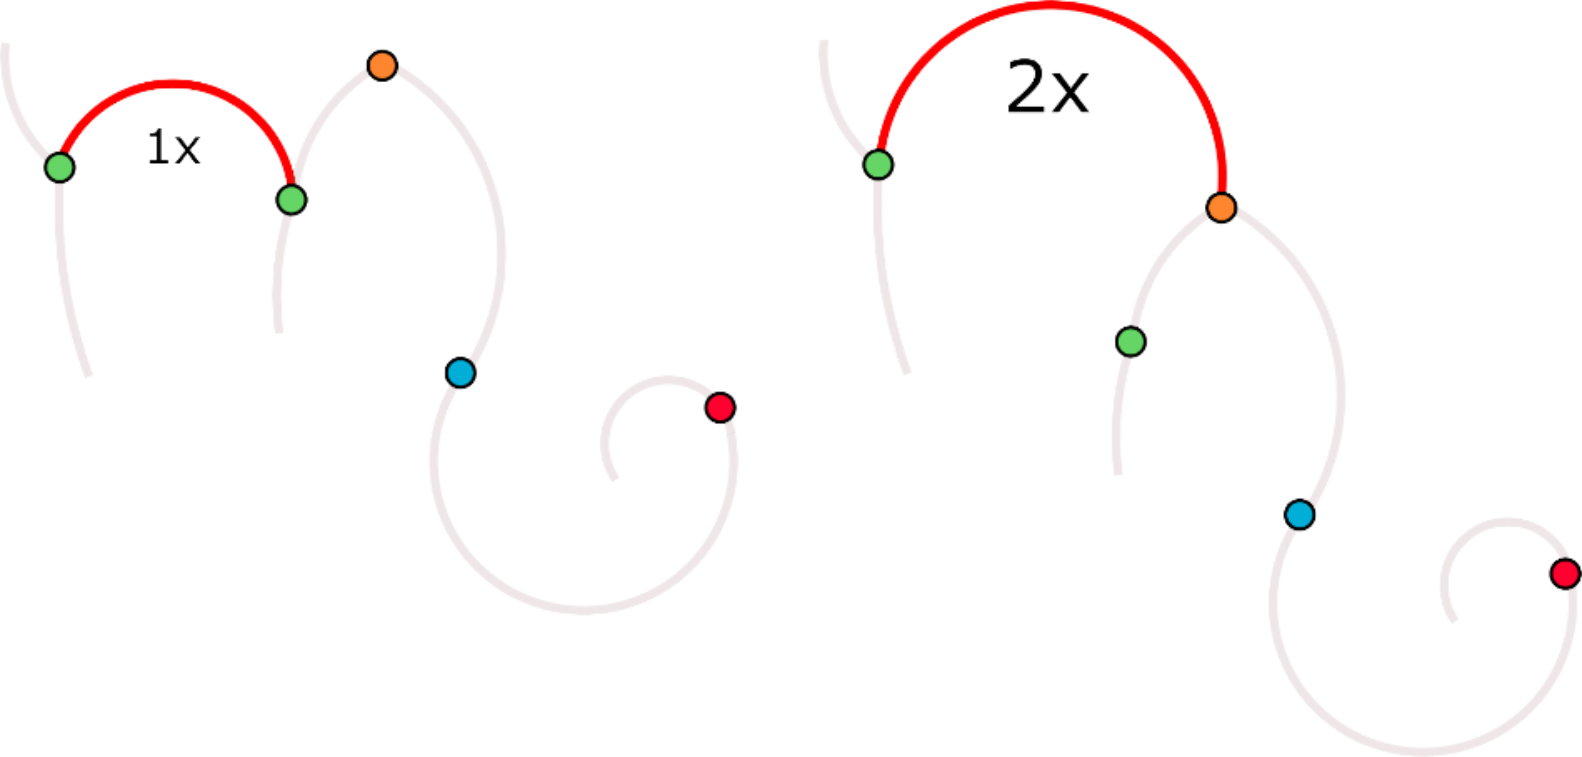
\includegraphics[width=0.85\linewidth,keepaspectratio]{images/metrics}
\caption{Геометрическая интерпретация изображений с метрикой}
\medskip
\small
На изображении видно как меняется геометрическое представление изображения, если меняется относительная длина дуги (красная дуга)
\end{figure*}

\item \textbf{Анализ изображения с использованием масштабных рядов} -- введение масштабных рядов предполагает введение вполне упорядоченного множества $ScaleLine$, которое соответствует масштабному ряду (аналог масштабного ряда топографических карт 1:500,  1:1000 и т.д.), а также два дополнительных отношения: $Scale$,  которое связывает дуги с элементами $ScaleLine$ и $Include$ которое связывает дугу $arc$ с ее образом $arc_1$ при сжатии изображения, т.е. при переходе к следующему (большему на единицу) элементу масштабного ряда.

Таким образом, совокупность всех дуг $A$ четырехосновной а.с.\ref{eq:model} может быть представлено в виде \begin{equation}
A = A_1 \cup A_2 \cup ... \cup A_n
\label{eq:components_set}
\end{equation}
где  множества $A_i$ состоят из дуг, относящихся к $i$ - му элементу масштабного ряда. Подраздел включает некоторые оценки для частных случае задачи в данной постановке.

\begin{figure*}[h]
\centering
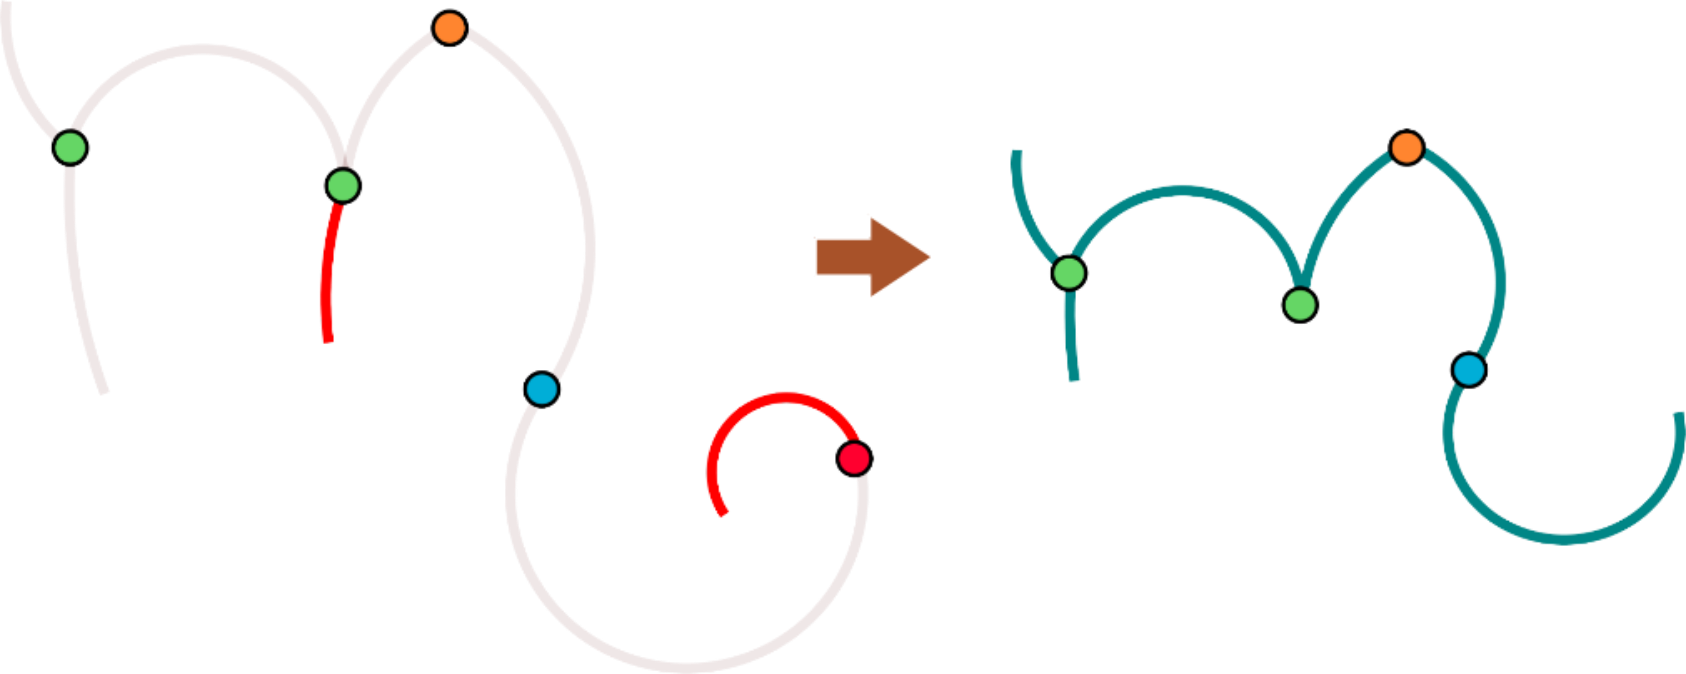
\includegraphics[width=0.85\linewidth,keepaspectratio]{images/scaleline}
\caption{Геометрическая интерпретация отмасштабированного изображения}
\medskip
\small
На изображении видно как одно и тоже изображение в разном масштабе может иметь разное количество дуг (незначимые в определенном масштабе дуги исчезают)
\end{figure*}


\item \textbf{Анализ изображений, представляющих объекты с наложениями} -- предполагает наличие объектов первого плана, отображенных на изображении без каких-либо искажений,  а также объектов второго и других планов, которые в той или иной степени закрыты более близко стоящими к точке съемки объектами. Схема поиска образцов второго плана состоит в проверке, что частично отображенные части каких-то образцов могут быть дополнены до всего образца дугами дерева решений (универсума), лежащими внутри  совокупности (объединения) образцов первого плана. В разделе доказывается следующая теорема: \begin{theorem}
Сложность поиска образцов первого, второго и любых других планов имеет верхнюю границу сложности не превышающую  
\begin{equation}
O((n+n)*n+m+n+(\psi*n*m)*n)
\label{overlaps:11}
\end{equation}
где  $\psi$ -- константа, соответствующая сложности проверки нахождения дуг из   внутри  образов найденных образцов (построенных изоморфными вложениями $\Sigma_1  =  \{\lambda_1, \lambda_2 ,..., \lambda_h\ \}$), где  $n$ -- верхняя граница на количество дуг и связей дуг у изображения и образцов,  $m$ -- количество образцов  $S_1, S_2, ..., S_m$.
\label{overlaps:t:5}
\end{theorem}   

\begin{figure*}[h]
\centering
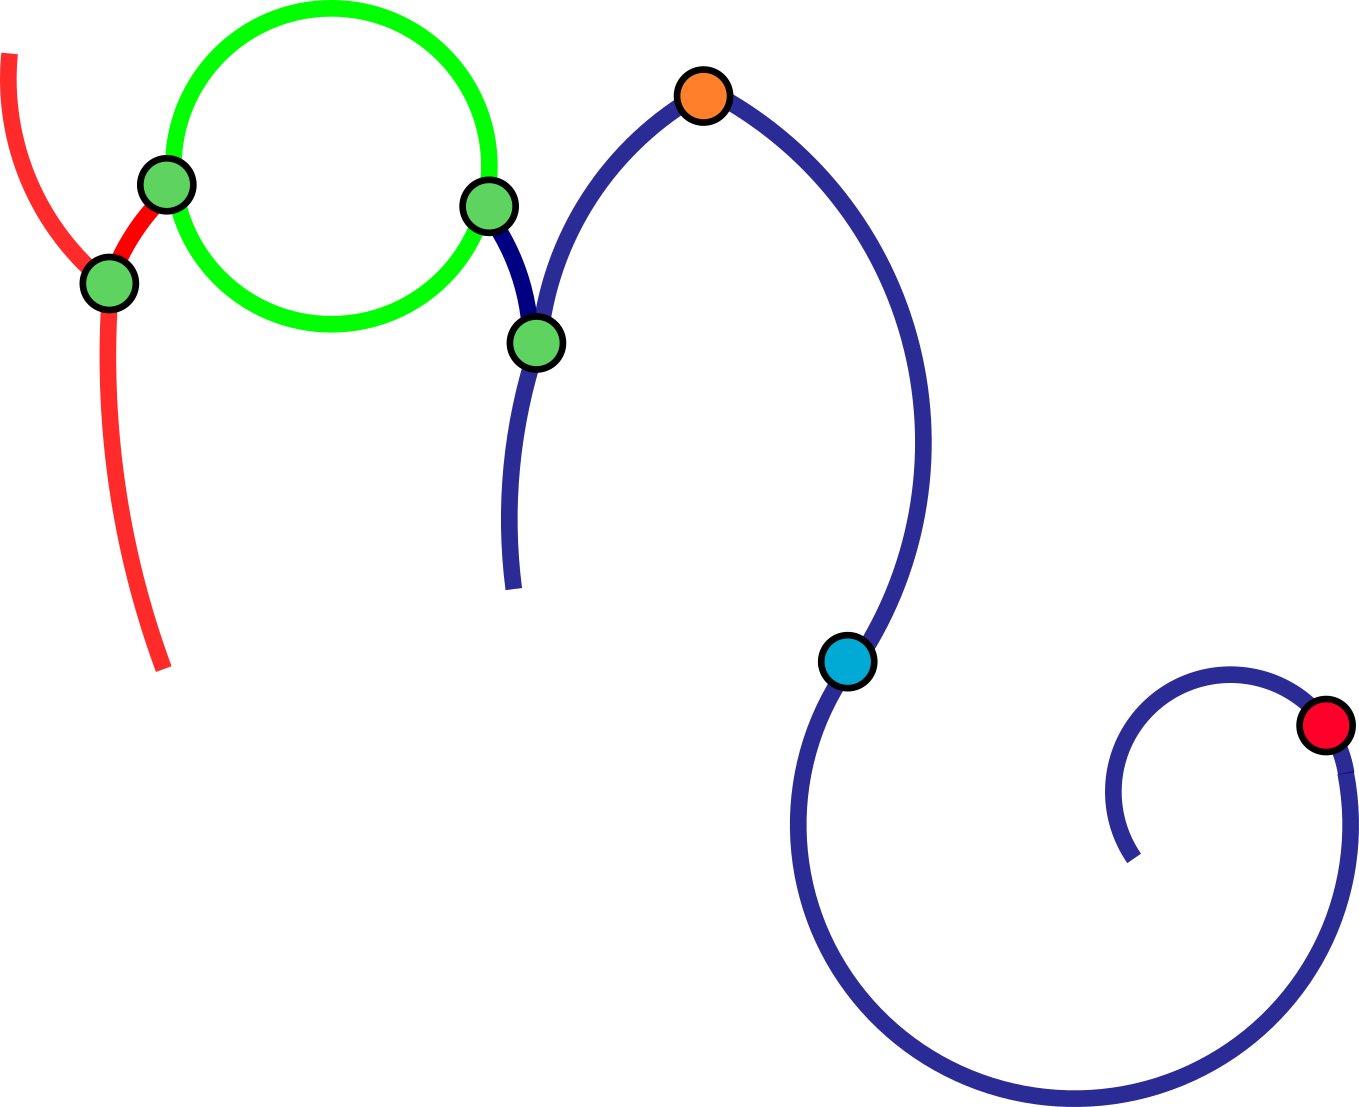
\includegraphics[width=0.55\linewidth,keepaspectratio]{images/overlaps}
\caption{Геометрическая интерпретация изображения с наложением}
\medskip
\small
На изображении видно как наложенное изображение первого плана (зеленое) разбивает исходный символ на два новых изображения второго плана
\end{figure*}
\end{enumerate}

\textbf{Третья глава} посвящена использования разработанных алгоритмов на практике и в производстве. Глава состоит из трех разделов.

В первом разделе описывается использование разработанного ПО для тестирования разработанных алгоритмов. Система состоит из трех модулей: конвертора растровых изображений (используется для наполнения БД тестовыми образцами), интерпретатор (для тестирования алгоритмов) и браузер базы данных. Программа написана на C++ и использует в качестве GUI Borland VLC.

Второй раздел посвящен применению разработанных алгоритмов в задаче оценки устойчивости битумных эмульсий. В отличие от задачи распознавания символов, здесь нет необходимости анализировать скелет изображения. Куда более важную роль играет внешний контур. Разбивая контур на дуги мы можем классифицировать частицы по уровню распада:
\begin{enumerate}
\item одиночные
\item слипшиеся
\item распавшиеся
\end{enumerate}
Большое количество распавшихся частиц является свидетельством того что смесь является неустойчивой, а следовательно некачественной.

В разделе описывается работа разработанной системы оценки морфологических характеристик частиц в битумных эмульсиях, а также построения распределений по этим данным.

\begin{figure}[h]
	\centering
	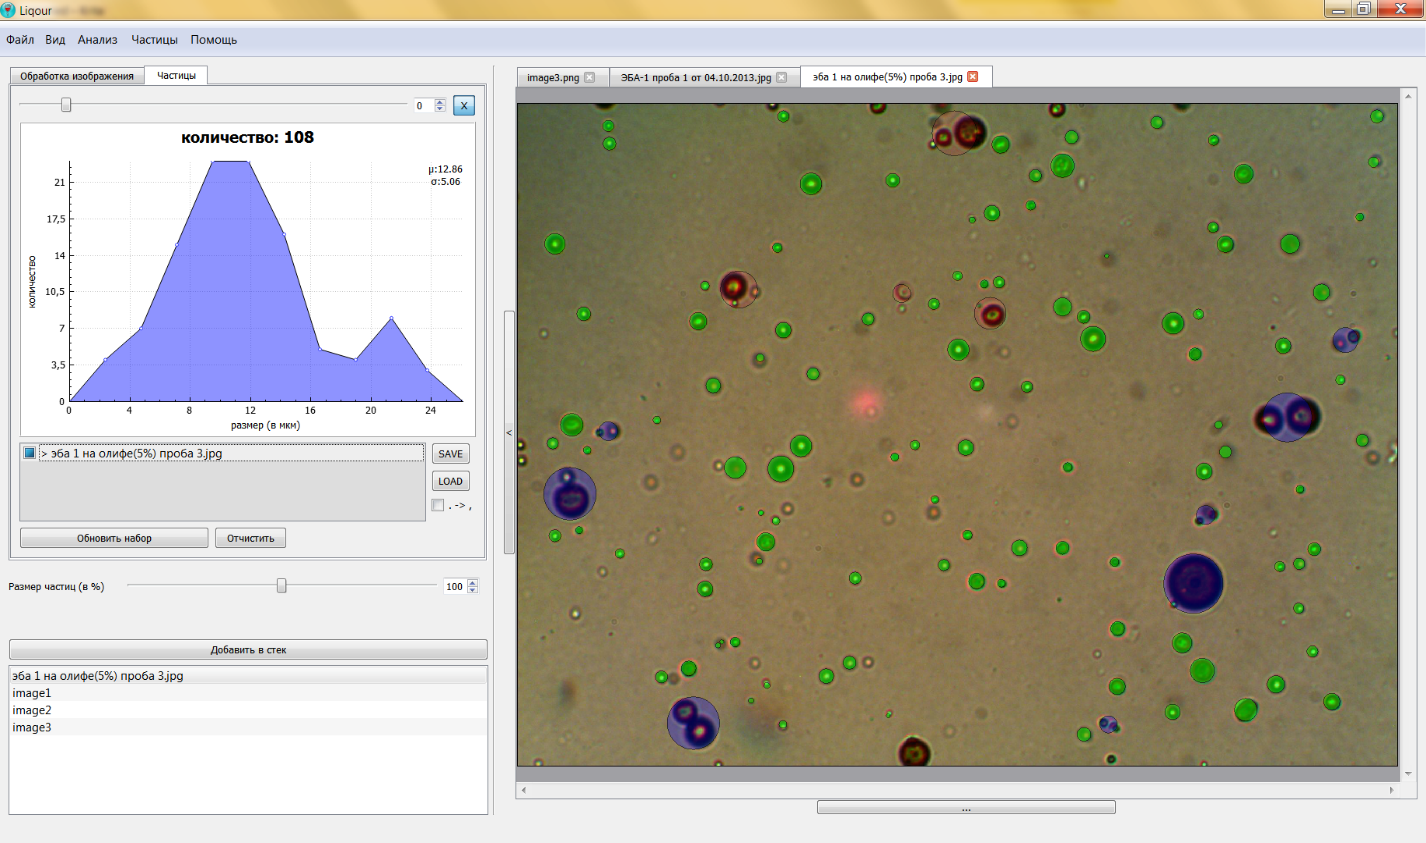
\includegraphics[scale=0.75]{images/em_05}
	\caption{ЭБА-1 на битуме разжиженном олифой (5\%)}
	\label{em_img_01}
\end{figure}

\begin{table}[h]
  \centering
  \caption{Распределение частиц на рис.\ref{em_img_01}}
  \renewcommand{\arraystretch}{1.5}% Spread rows out...Рис.9 Эмульсия, полученная в заводских условиях на вязком битуме.
  \begin{tabular}{*2{>{\centering\bfseries}m{1in}}>{\centering\arraybackslash}m{0.6in}}
    \toprule
	\textbf{Среднее значение, мкм.} & \textbf{Ср.кв. отклонение, мкм.} & \textbf{Всего частиц} \\
	\midrule
		\midrule
	12.86 & 5.06 & 108 \\
	\bottomrule
  \end{tabular}
  \label{em_table}
\end{table}

На рисунке \ref{em_img_01} представлен интерфейс программы, а в таблице \ref{em_table} также сравнение полученных результатов с реальными результатами.

Третий раздел посвящен применения методов интерпретации для задачи автоматизации составления проекта организации дорожного движения. В тексте предложена реализацию надстройки над базой данных, которая позволяет решать проверку удовлетворения расположения объекта на линейном графике набору ограничений, который в данном случае представленны формализованными ГОСТами.



В \textbf{заключении} приведены основные результаты работы, которые заключаются в следующем:
На качественном уровне: для данных, организованных более сложно, чем  таблицы реляционных баз данных, доказаны очень близкие результаты по вычислительной сложности их анализа.
Более точно, основные результаты работы могут быть сформулированы следующим образом.
\begin{enumerate}
\item На основе анализа плоских контурных изображений разработана формализация, представленная ориентированными дугами, связями дуг и их численными характеристиками в градусном измерении и  относительными размерами  длины дуг.
\item Исследования показали, что вычислительная сложность  анализа плоских контурных изображений, представленных ориентированными дугами, связями дуг и их численными характеристиками в градусном измерении и  относительными размерами  длины дуг, почти не зависит от количества образцов.
\item Для подтверждения теоретических результатов на практике  было созданы комплексы программ для решения задач.
\end{enumerate}


\def\selectlanguageifdefined#1{
\expandafter\ifx\csname date#1\endcsname\relax
\else\language\csname l@#1\endcsname\fi}
\ifx\undefined\url\def\url#1{{\small #1}}\else\fi
\ifx\undefined\BibUrl\def\BibUrl#1{\url{#1}}\else\fi
\ifx\undefined\BibAnnote\long\def\BibAnnote#1{(#1)}\else\fi
\ifx\undefined\BibEmph\def\BibEmph#1{\emph{#1}}\else\fi

\renewcommand{\refname}{Список основных работ по теме диссертации}
\begin{thebibliography}{10}

\bibitem{D15}
\selectlanguageifdefined{russian}
Мартьянов~В.И., Архипов~В.В., Каташевцев~М.Д.
  {[и~др.]}; Обзор приложений
  логико-эвристических методов решения
  комбинаторных задач высокой сложности~//
  Современные технологии. Системный анализ.
  Моделирование. ИрГУПС.
\newblock 2010.
\newblock Т. №4(28).
\newblock {С.}~61--67.{}

\bibitem{D19}
\selectlanguageifdefined{russian}
Комбинаторные задачи высокой сложности и
  анализ плоских контурных изображений~/
  В.И.~Мартьянов, М.Д.~Каташевцев~// Известия
  Иркутского Государственного
  Университета серия <<Математика>>.
\newblock 2013.
\newblock Т. №4.
\newblock {С.}~31--47.{}

\bibitem{scaleline}
\selectlanguageifdefined{russian}
Масштабные ряды плоских контурных
  изображений и их применение.~/
  В.И.~Мартьянов, М.Д.~Каташевцев~// Вестник
  ИрГТУ.
\newblock 2016.
\newblock Т. №5(99).
\newblock {С.}~121--129.{}

\bibitem{overlaps}
\selectlanguageifdefined{russian}
Анализ плоских контурных изображений,
  представляющих объекты с наложениями.~/
  В.И.~Мартьянов, М.Д.~Каташевцев~// Вестник
  ИрГТУ.
\newblock 2017.
\newblock Т. №1(120).
\newblock {С.}~63--71.{}

\bibitem{D18}
\selectlanguageifdefined{russian}
Свидетельство о
  государственной регистрации программы
  для ЭВМ №2011618417  / М.Д~Каташевцев, В.И.~Мартьянов~// Федеральная служба по
    интеллектуальной собственности, патентам
    и товарным знакам.- Москва. -- 2010. (авторский объём – 75\%).

\bibitem{D6}
\selectlanguageifdefined{russian}
Волновая скелетизация~/ М.Д.~Каташевцев~//
  Вестник Иркутского Государственного
  Технического Университета.
\newblock 2013.
\newblock Т. №7.
\newblock {С.}~89--92.{}

\bibitem{D8}
\selectlanguageifdefined{russian}
Анализ плоских контурных изображений с
  метрикой~/ М.Д.~Каташевцев~// Известия
  Иркутского Государственного
  Университета серия <<Математика>>.
\newblock 2014.
\newblock Т. №9.
\newblock {С.}~39--48.{}

\bibitem{D7}
\selectlanguageifdefined{russian}
Каташевцев~М.Д., Мартьянов~В.И.,
  Степаненко~А.А. {[и~др.]};
  Автоматизированная технология создания
  проектов организации дорожного
  движения~// Вестник ИрГТУ.
\newblock 2012.
\newblock Т. №10(69).
\newblock {С.}~150--155.{}

\bibitem{emulsion}
\selectlanguageifdefined{russian}
Каташевцев~М.Д., Алексеенко~В.В., Воронов~Д.В.
  {[и~др.]}; Исследование гранулометрического
  состава эмульсий с помощью оптического
  микроскопа и методом автоматизированного
  распознавания объектов на цифровой
  фотографии~// Вестник ИрГТУ.
\newblock 2015.
\newblock Т. №2.
\newblock {С.}~99--103.{}

\bibitem{D20}
\selectlanguageifdefined{russian}
Пахомов~Д.В., Каташевцев~М.Д., Мартьянов~В.И.
  {[и~др.]}; Автоматизация создания проектов
  организации дорожного движения для
  автомобильных дорог~// Современные
  технологии. Системный анализ.
  Моделирование. ИрГУПС.
\newblock 2010.
\newblock {С.}~56--61.{}

\centerline{\textbf{Публикации в других издания}}

\bibitem{D5}
\selectlanguageifdefined{russian}
Логико-эвристические методы анализа
  плоских изображений~/ М.Д~Каташевцев,
  В.И.~Мартьянов~// Известия Иркутского
  университета: ежегод.науч.-теорет. конф.
  аспирантов и студентов: материалы. –
  Иркутск: Изд-во Иркут. гос.ун-та,.
\newblock 2010.
\newblock {С.}~175--177.{}

\bibitem{D26}
\selectlanguageifdefined{russian}
Мартьянов~В.И., Архипов~В.В., Каташевцев~М.Д.
  {[и~др.]}; Обзор приложений
  логико-эвристических методов решения
  комбинаторных задач~// Материалы 3-ей
  Российской школы – семинара «Синтаксис и
  семантика логических систем».- Иркутск.
\newblock 2010.
\newblock {С.}~60--64.{}

\end{thebibliography}


\vfill
\pagenumbering{gobble}
\begin{center}
Подписано в печать 07.10.2017. Формат 60 $\times$ 90 /16.

Бумага офсетная. Печать цифровая. Усл. печ. л. 1,0.

Тираж 100 экз. Заказ 241. Поз. Плана 8н.
\bigskip

Отпечатано в типографии издательства

ФГБОУ ВО «Иркутский национальный 

исследовательский технический университет»

664074, г. Иркутск, ул. Лермонтова, 83.
\end{center}